\section{Alpha-beta search}

\begin{enumerate}
    \item Perform the MiniMax algorithm on the tree in Figure 1, i.e. put a value to each node. Circle the move the root player should do.
      \begin{figure}[!ht]
      \begin{framed}
	  \centering
	  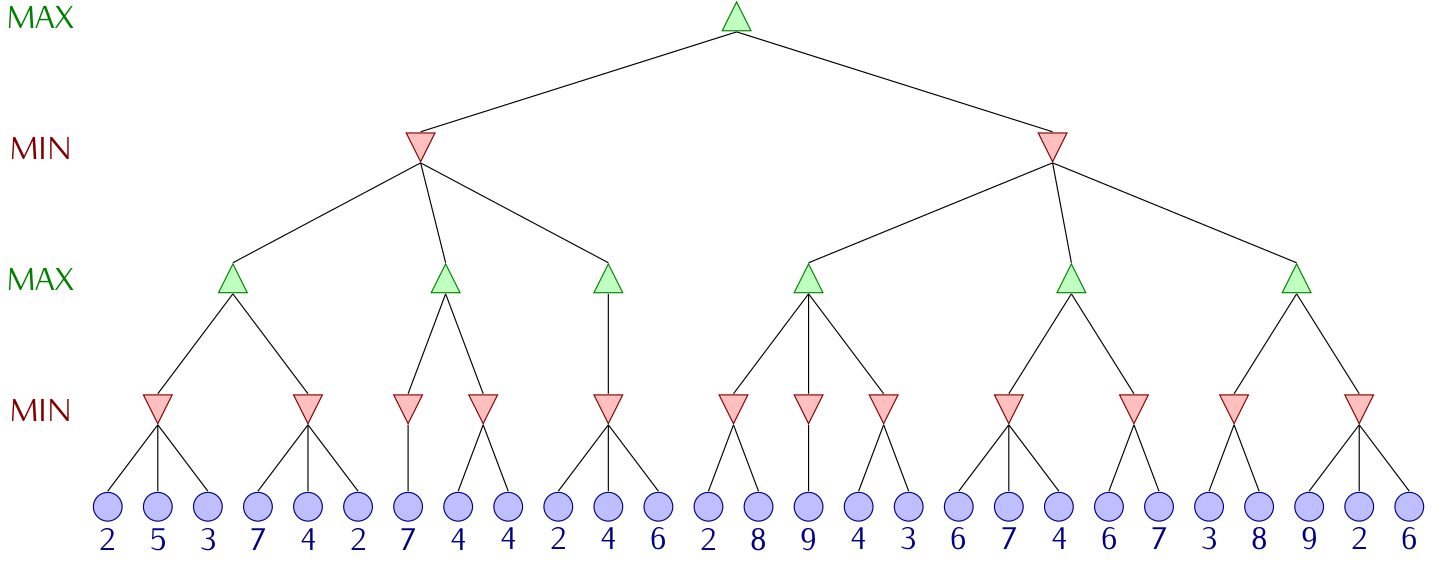
\includegraphics[width=\linewidth]{tree.png}
	  \caption{MiniMax}
      \end{framed}
      \end{figure}
      \FloatBarrier
    \item Perform the Alpha-Beta algorithm on the tree in Figure 2. At each non terminal node, put the successive values of $\alpha$ and $\beta$. Cross out the arcs reaching non visited nodes. Assume a left-to-right node expansion.
      \begin{figure}[!ht]
      \begin{framed}
	  \centering
	  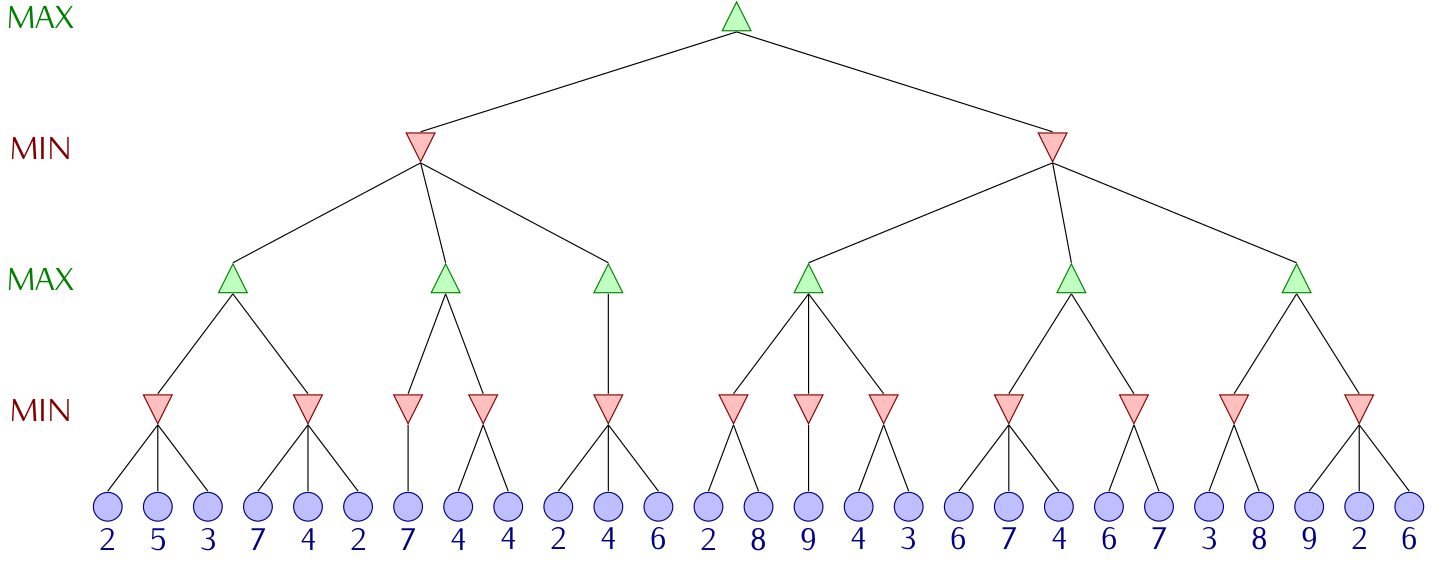
\includegraphics[width=\linewidth]{tree.png}
	  \caption{Alpha-Beta, left-to-right expansion}
      \end{framed}
      \end{figure}
      \FloatBarrier
    \item Do the same, assuming a right-to-left node expansion instead (Figure 3).
      \begin{figure}[!ht]
      \begin{framed}
	  \centering
	  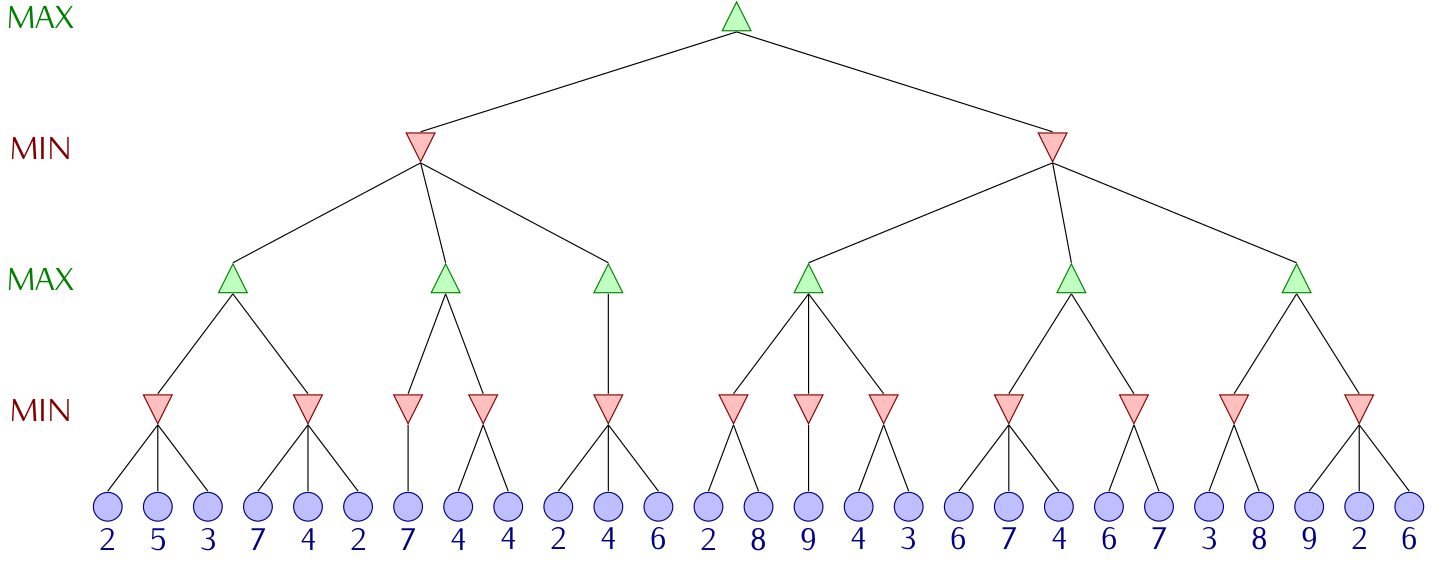
\includegraphics[width=\linewidth]{tree.png}
	  \caption{Alpha-Beta, right-to-left expansion}
      \end{framed}
      \end{figure}
      \FloatBarrier
    \item Can the nodes be ordered in such a way that Alpha-Beta pruning can cut off more branches (in a left-to-right node expansion)? If no, explain why; if yes, give the new ordering and the resulting new pruning.
      \begin{figure}[!ht]
      \begin{framed}
        The nodes can be ordered in such a way that Alpha-Beta pruning can
        cut off more branches, as shown in the following tree:

        \bigskip
        \bigskip
	  \centering
	  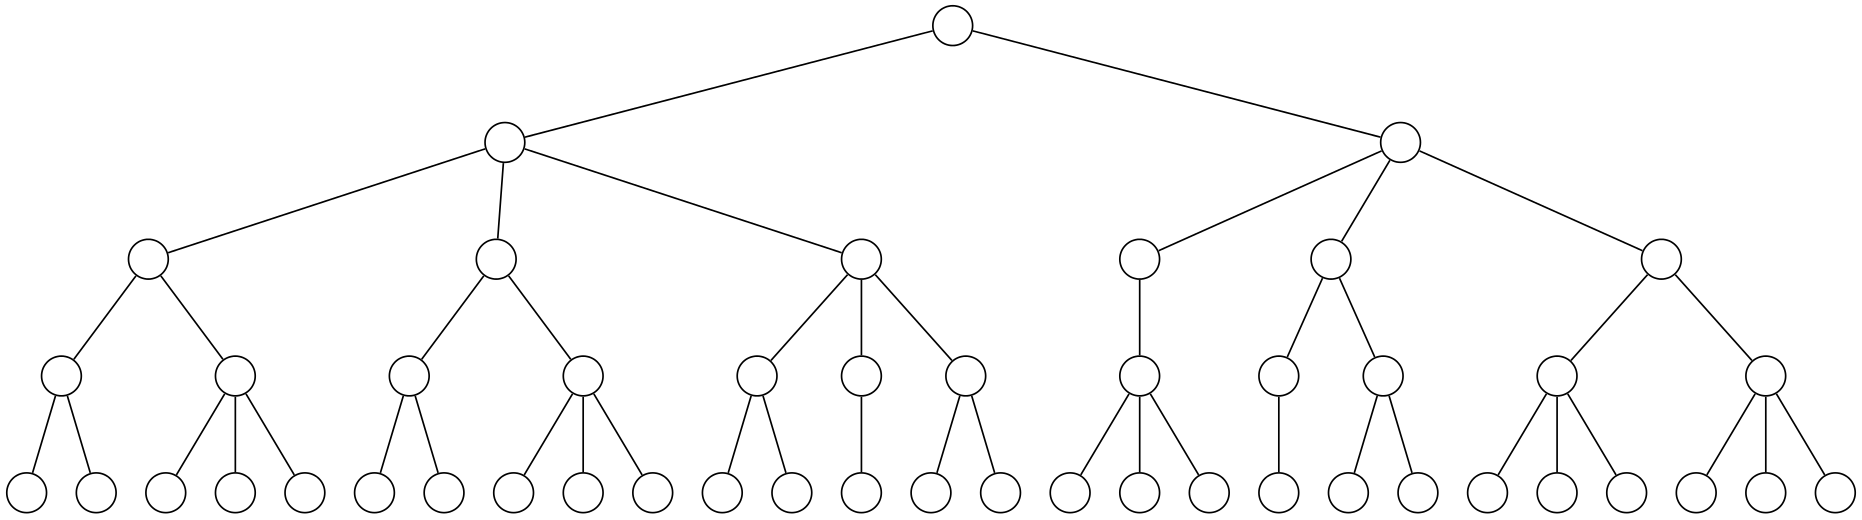
\includegraphics[width=\linewidth]{my_tree.png}
      \bigskip
      \bigskip
	  \caption{Alpha-Beta, left-to-right expansion on ordered tree}
      \end{framed}
      \end{figure}
      \FloatBarrier
\end{enumerate}

\section{Avalam}
    \subsection{A basic alpha beta agent}
    \subsection{Comparison of two evaluation functions}
    \begin{enumerate}
    \item[6.] Launch a game where one of the agents is the basic agent described before against another agent where the basic evaluate method has been replaced such that it returns directly the result of Board.get\_score instead of -1, 0 or 1. Watch the replay of the match. What do you observe? Does one of the agent clearly overcomes the other one? Explain why there is such a difference.
      \begin{framed}
          When the new version of basic agent is Player 1, it clearly
          overcomes the old version because even with a depth of 2, the
          differences between the values evaluated are  much more relevant.
          \newline

          When the new version of basic agent is Player 2, the old basic
          agent wins because the improvement does not overcome the advantage
          from being Player 1. The first moves aren't very good but it gets
          better and better as the game enfolds catching back nearly all
          its delay at the end, losing by only 1 point. \newline
      \end{framed}
\end{enumerate}

\subsection{Evaluation function}

    \begin{enumerate}
        \item[7.] Describe precisely your evaluation function.
        \begin{framed}
            In our evaluation fonction, we first start by separating the board positions in three types. If the position is empty we ignore it. If the position is filled a tower of height five, we add (or substract depending on the color of the tower) a fixed score X to the total score of the board. Finally for every positions that doesn't fit the two previous criteria we call the towerScore method. \newline

            In this towerScore fonction, we calculate the score that should be allowed to the tower depending to various factor. First, if the tower is isolated, we return a fixed score Y such as X > Y, allowing our algorithm to prefer state with more tower of height five than others. The difference is of course not too large so that the algorithm doesn't sacrifice two isolated tower for a tower of height five. \newline

            If the tower isn't isolated, the algorithm will then determine if the tower is in a simple snapback state wich we define as follow : If a tower of height one or two doesn't have an ally of the same color on which it could jump on and if for every ennemy it could jump on the ennemy can either form a tower of height five or an isolated tower with his next move, then the tower is in a simple snapback state. \newline

            Of course some pure snapback states are not contained in this description but it was necessary for the evaluation method to run as fast as possible so we kept only the most common and obvious definition of a snapback to speed it up. The other snapack states will still usually be found as the depth increases, but this gives us a safety margin for lower depth computation. \newline

            Finally if the tower is neither isolated nor in a snapback state, we return a given score depending on the height of the tower at hand. This score is such that a tower of height 1 is worth more than a tower of height 2 which is worth more than a tower of height three or four. Doing so allows our algorithm to reduce the opponent's possibilites if an occasion to do so arises. \newline

            When our algorithm has computed the score for each position of the board, adding or substracting it depending on the color, we simply return this score as the evaluation of the board. \newline
        \end{framed}
    \end{enumerate}

\subsection{Successors function}

\begin{enumerate}
    \item[8.] Give an upper and a lower bound on the branching factor for a search tree on the Avalam game. Justify your answer.
    \begin{framed}
        For an algorithm that doens't drop branches, we can easily differ that the branching factor will be lower as the game enfolds because every step consume a tower thus the number of action possible keeps decreasing. We can thus easily affirm that the branching factor will be comprised between 292 which is the branching factor of a brand new game and 2 which is the lowest branching factor that could happen for the last move when only two movable towers are left next to each other. The branching factor is thus comprised in the domain $[2, 292]$
    \end{framed}
    \item[9.] How does the branching factor evolve after a move has been performed? Explain.
    \begin{framed}
        As explained in the previous answer, it will decrease at each step but the quantity by which it decreases is variable as it depends on the neighbours of the moved tower.
    \end{framed}
    \item[10.] Can you think of states that might be ignored? What do you loose if you ignore successors? Explain.
    \begin{framed}
        There is quite a number of states that could potentially be ignored but doing so might not always be safe as it could drop with it potential for better states. For example, a move that can be safely dropped is when two tower which fill each other are next to each other, we can safely ignore states where the current player give a five tower to the ennemy by making an ennemy tower jump on his tower. \newline

        Similarly we can drop moves where the current player isolate a tower for the ennemy but it might not be safe as giving that tower to the ennemy may allows us to make more points later on. Dropping tower is thus a dangerous but worthy gamble.
    \end{framed}
    \item[11.] Describe your successors function.
    \begin{framed}
        Our successor function is quite simple, we simply call the get\_sorted\_action() method which does the same as the original get\_actions() except that it sorts the actions it returns so that the most interesting ones tend to be yield towards the beginning. It will also drops extremely useless possibilities like a one surrounded by seven or more ones other ones.

        It then plays those action on a clone of the old board and yields the resulting new boards in succession
    \end{framed}
\end{enumerate}

\subsection{Cut-off function}

\begin{enumerate}
    \item[12.] The \verb#cutoff# method receives an argument called depth . Explain precisely what is called the \textit{depth} in the \verb#minimax.py# implementation.
    \begin{framed}
        The depth argument is the current depth at which the minmax function is in the search tree. Thus the root will be at depth 0, its branches will be at the two and so forth and so on.
    \end{framed}
    \item[13.] Explain why it might be useful (for the Avalam contest) to cut off the search for another reason than the depth. Would it be interesting to consider a changing cutoff function (i.e. it changes according to the advancement of the game).
    \begin{framed}
        It might be usefull if our algorithm takes too much time to compute a given depth, interrupting the execution and allowing for it to recompute at a lower depth may be wiser than keep going on and wasting lots of time credit. \newline

        Changing the depth depending on the game state would be an excellent decision (which we also implemented) as the time to compute a given depth will be reduced as the game enfolds. As such a depth 2 which took 6 seconds at the beginning of the game might take only half a second at step 20. Implementing a changing cutoff function is thus a must have for the contest as seeing deeper allows an algorithm to perform better results.
    \end{framed}
    \item[14.] Describe your cut-off function.
    \begin{framed}
        Our cutoff function will use a precomputed maximum depth and a precomputed maximum time to run and proceeds as follow :

        \begin{itemize}
            \item A computation with a \textbf{depth lower than 3} will always wait to finish and will never be interrupted due to a lack of time as we consider that we need at least that to play a decent move.
            \item If the \textbf{depth is bigger than 2 and we aren't in lack of time}, cutoff will only return true if the current depth equals the maximum allowed depth that we precomputed earlier.
            \item If the depth is \textbf{bigger than 2 but we exceeded our decided time limit} for this step, our algorithm will process the rest of the tree in depth 2 to avoid wasting too much time. We infered after much reflexion that it would be better to play a good move where we have fully seen the outcome rather than playing blind and see what happens but it is also better to play blind than to play what we know is a bad move. Thus this seemed to be the best solution and this works normally well with our algorithm as we reorder the subtree in such a way that the most interesting actions will be tested toward the beginning.
        \end{itemize}
    \end{framed}
\end{enumerate}

\subsection{A Smart Alpha-Beta Agent}

\begin{enumerate}
    \item[15.] Upload your agent to the INGInious \textit{Assignment 3 - Avalam: Super Agent} task. Your agent will play a match against a simple alpha-beta player. Each agent will have a time credit of 2 . 5 minutes. If you win against this agent, you get all the points for the question. If you succeed to perform a draw, you get half of the points and if get beaten, you don’t get any point. Don’t forget to include all the needed files inside the archive you upload.
    \begin{figure}[!ht]
    \begin{framed}
        \centering
        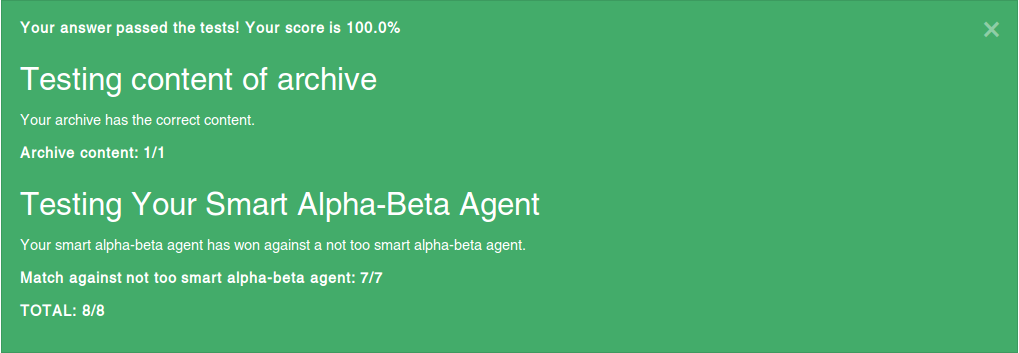
\includegraphics[width=\linewidth]{test_super_agent.png}
        \caption{INGInious result on super agent}
    \end{framed}
    \end{figure}
\end{enumerate}

\subsection{Contest}

\begin{enumerate}
    \item[16.] Upload your agent to the INGInious \textit{Assignment 3 - Avalam: Contest Agent} task. Your agent will play a match against a basic alpha-beta player. Each agent will have a time credit of 2 . 5 minutes (for the real contest, your agent will have a time credit of 20 minutes per match). If you win against this agent, you get all the points for the question. If you succeed to perform a draw, you get half of the points and if get beaten, you don’t get any point. Don’t forget to include all the needed files inside the archive you upload.
        \begin{figure}[!ht]
        \begin{framed}
            \centering
            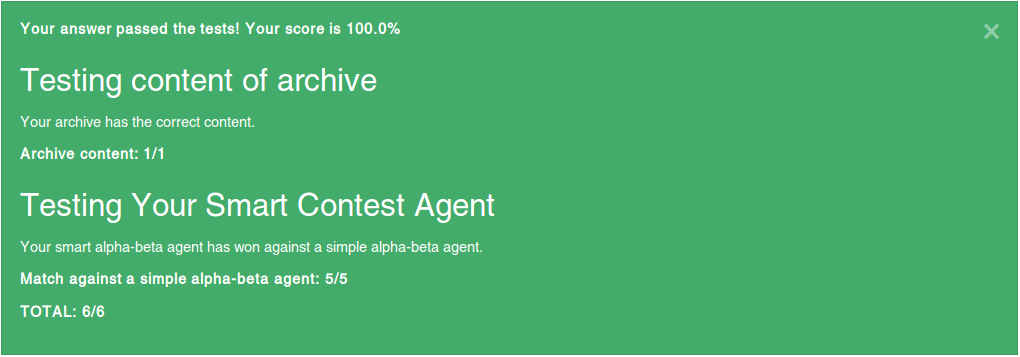
\includegraphics[width=\linewidth]{test_contest_agent.png}
            \caption{INGInious result on contest agent}
        \end{framed}
        \end{figure}
    \item[17.] Describe concisely your super tough agent in your report. \textbf{Your description shouldn’t be longer than one A4 paper page; if it is the same agent than the one described in earlier sections, just state it, no need to re-explain.}
    \begin{framed}
        Our super tough contest performs the same behaviour we described previously in this report. There is however a feature in our code that we didn't have the occasion to mention previously. \newline

        When our board execute the minimax function, it saves at each steps the combinaison of moves that lead to that given state to avoid visiting symmetric boards.
    \end{framed}
\end{enumerate}
